\textbf{Входные параметры:}
 
 Fitness --- массив пригодностей индивидов;
 
 SizeTournament --- размер турнира;
 
 VMHL\_N --- размер массива.

\textbf{Возвращаемое значение:} 

 Номер выбранного индивида популяции.

 Для переопределенной функции.
 
 \textbf{Входные параметры:}
 
 Fitness --- массив пригодностей индивидов;
 
 SizeTournament --- размер турнира;
 
 Taken --- Информация о том, в турнире или нет индивид (служебный массив);
 
 VMHL\_N --- размер массива.

\textbf{Возвращаемое значение:} 

 Номер выбранного индивида популяции.
 
 \textbf{Примечание:}

 Является стандартной реализацией турнирной селекции. Это турнирная селекция без возвращения.
 
 \begin{figure} [h]
  \center
  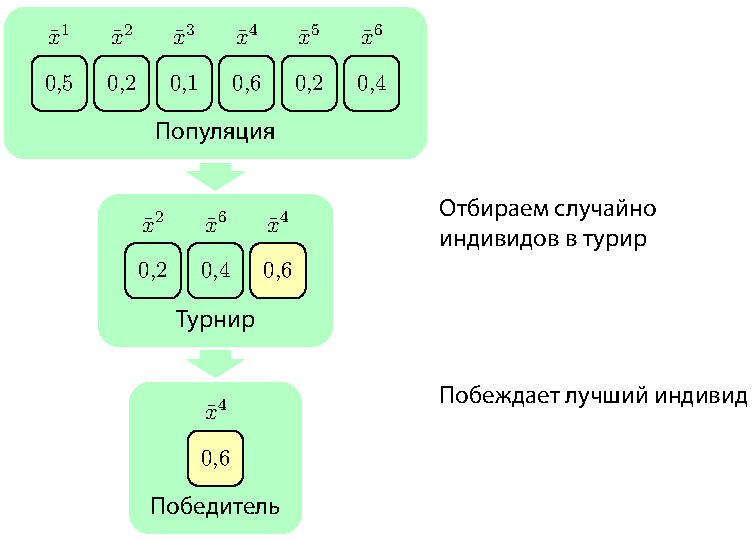
\includegraphics [scale=0.8] {MHL_TournamentSelection_Sheme}
  \caption{Механизм работы турнирной селекции} 
  \label{img:MHL_TournamentSelection_Sheme}  
\end{figure}

